\documentclass[a4paper,10pt]{article} % type, taille police

\usepackage[utf8]{inputenc} % encodage
\usepackage[T1]{fontenc} % encodage
\usepackage[french]{babel} % gestion du français
\usepackage{amssymb} % symboles mathématiques
\usepackage{textcomp} % flèche,  intervalle
\usepackage{stmaryrd} % intervalle entiers

\usepackage[left=3cm,right=3cm,top=3cm,bottom=3cm]{geometry} % marges
\usepackage[hidelinks]{hyperref} % sommaire interactif dans un pdf
\usepackage[nottoc, notlof, notlot]{tocbibind} % affichage des références dans la table des matières (?)
\usepackage{float} % placement des figures
\usepackage[toc,page]{appendix} % ajout d'annexes
\usepackage{amsthm} % format des déf, prop...
\usepackage{amsmath} % matrices, ...
\usepackage{multirow} % fusionner cellules verticalement

%\usepackage[french,ruled,vlined,linesnumbered]{algorithm2e} % affichage d'algorithmes
\usepackage{tikz} % affichage de schémas
\usepackage{graphicx} % affichage d'images
\usepackage{url} % inclure des urls
\usepackage{bbold} % fonction caractéristique 1

\renewcommand{\appendixtocname}{Annexes} % renommage annexes
\renewcommand{\appendixpagename}{Annexes}

%\providecommand{\SetAlgoLined}{\SetLine} % paramètre pour algorithm2e
%\providecommand{\DontPrintSemicolon}{\dontprintsemicolon}  % paramètre pour algorithm2e

\definecolor{bgreen}{rgb}{0.30,0.70,0}

\theoremstyle{definition} % pas d'italique pour le format des déf, prop...
\newtheorem{thm}{Théorème} % \begin{thm} \end{thm}
\newtheorem{cor}[thm]{Corollaire}
\newtheorem{defi}[thm]{Définition}
\newtheorem{ex}[thm]{Exemple}
\newtheorem{lem}[thm]{Lemme}
\newtheorem{rem}[thm]{Remarque}
\newtheorem{conj}[thm]{Conjecture}

\newcommand{\R}{\mathbb{R}}
\newcommand{\Q}{\mathbb{Q}}
\newcommand{\N}{\mathbb{N}}
\newcommand{\Z}{\mathbb{Z}}
\newcommand{\inorm}[2]{{\left\lVert{#1}\right\rVert_{#2}}}
\newcommand{\infnorm}[1]{\inorm{#1}{}}
\newcommand{\clength}[1]{\operatorname{length}(#1)}
\newcommand{\twonorm}[1]{\inorm{#1}{2}}
\newcommand{\gpacrec}{R_{GPAC}}
\newcommand{\gpacpoly}{P_{GPAC}}
\newcommand{\gpacnpoly}{NP_{GPAC}}
\newcommand{\gpacspace}{PSPACE_{GPAC}}

%#############################################################################################################%
%#############################################################################################################%
%#############################################################################################################%

\title{Reconnaissance et indexation de formes}
\author{Quentin Cormier \and Yassine Hamoudi}
\date{4 mai 2015}

\begin{document}

\maketitle

\tableofcontents

%#############################################################################################################%
%#############################################################################################################%
%#############################################################################################################%

\section{Introduction}

%#############################################################################################################%
%#############################################################################################################%
%#############################################################################################################%

\section{Méthode}

% mettre des exemples d'images après normalisation

%#############################################################################################################%
%#############################################################################################################%
%#############################################################################################################%

\section{Résultats}

Nous exposons les résultats obtenus grâce à la méthode détaillée précédemment. Nous allons étudier dans un premier temps la sensibilité de notre algorithme aux perturbations (rotation, redimensionnement, bruit, ...), puis nous détaillerons les résultats de classification sur le dataset d'images.

%-------------------------------------------------------------------------------------------------------------%

  \subsection{Sensibilité aux perturbations}

Les valeurs propres du Laplacien de Dirichlet vérifient un certain nombre de propriétés mathématiques qui garantissent que notre descripteur est insensible au redimensionnement, à la rotation et à la translation. Nous vérifions expérimentalement ces propriétés ci-dessous.

~\\
\underline{Redimensionnement} Etant donné un domaine $\Omega$ et un facteur $a > 0$, on a $\lambda_k(a \Omega) = \frac{\lambda_k(\Omega)}{a^2}$ (voir \cite{KhabouHR07}). Or, notre descripteur utilise des rapports de valeurs propres, il est donc inchangé par redimensionnement : $\frac{\lambda_k(a \Omega)}{\lambda_m(a \Omega)} = \frac{\lambda_k(\Omega)}{\lambda_m(\Omega)}$. Nous avons calculé différents rapports pour l'image \texttt{camel-1.pgm}, les résultats figurent table \ref{scale}. Les variations d'une image à l'autre peuvent s'expliquer par les dégrations des contours suite au redimensionnement. Les rapports restent tout de même très proches. En pratique, nous utilions une longueur de 50 pixels afin d'obtenir des temps de calcul raisonnables (environ 20s pour calculer les valeurs propres associées à une image de taille 50x50).

\begin{table}[H]
  \begin{center}
    \begin{tabular}{l | c c c c c c}
                & $\lambda_1 / \lambda_2$ & $\lambda_1 / \lambda_3$ & $\lambda_1 / \lambda_4$ & $\lambda_2 / \lambda_3$ & $\lambda_3 / \lambda_4$ & $\lambda_4 / \lambda_5$ \\ \hline
      75 pixels & 0.63 & 0.42 & 0.36 & 0.67 & 0.84 & 0.89 \\
      50 pixels & 0.61 & 0.42 & 0.32 & 0.68 & 0.83 & 0.89 \\
      25 pixels & 0.53 & 0.39 & 0.31 & 0.73 & 0.80 & 0.81
    \end{tabular}
  \end{center}
\caption{Rapports de valeurs propres en fonctions de la longueur de l'image \texttt{camel-1.pgm} redimensionnée (l'image initiale est de taille 346x346)}
\label{scale}
\end{table}

~\\
\underline{Translation} Nous recadrons systématiquement l'image afin de conserver le plus petit rectangle contenant la figure. Ceci nous permet d'être insensible aux translations.

~\\
\underline{Rotation} Il a été démontré mathématiquement que les valeurs propres sont inchangées lorsque le domaine subit une rotation (voir \cite{Zuliani04}). Ce résultat se vérifie facilement à partir de quatre rotations appliquées sur \texttt{deer-20.pgm}. Les valeurs propres associées à chaque figure sont regroupées dans la table \ref{rot}.

\begin{center}
  \begin{tabular}{c c c c}
    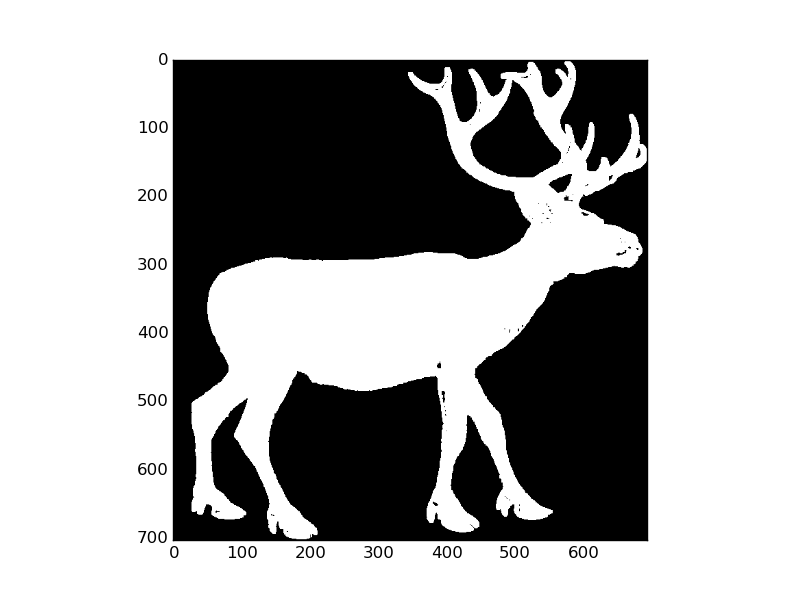
\includegraphics[scale=0.15]{rotate/0.png} & 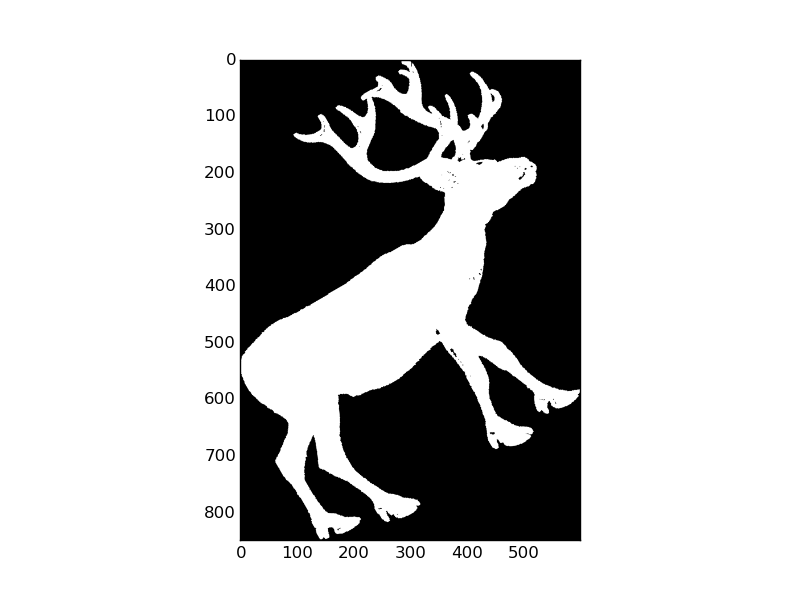
\includegraphics[scale=0.15]{rotate/30.png} & 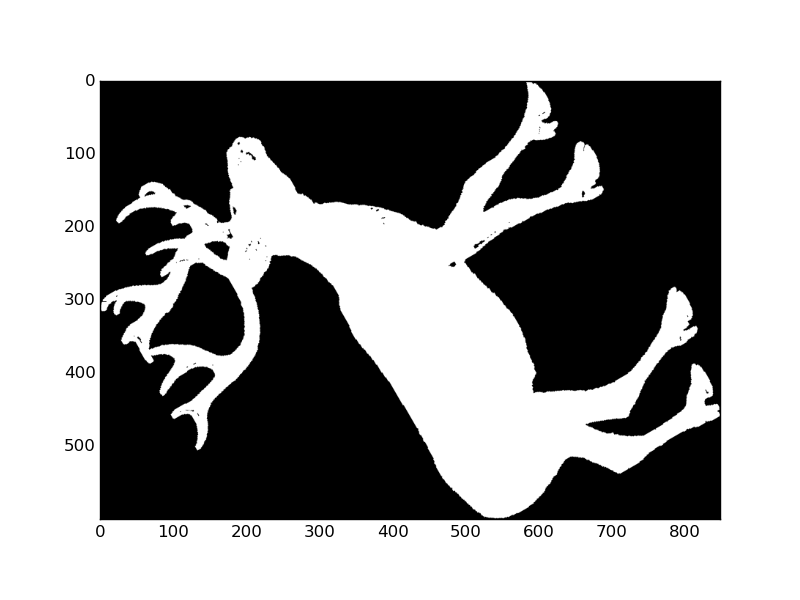
\includegraphics[scale=0.15]{rotate/120.png} & 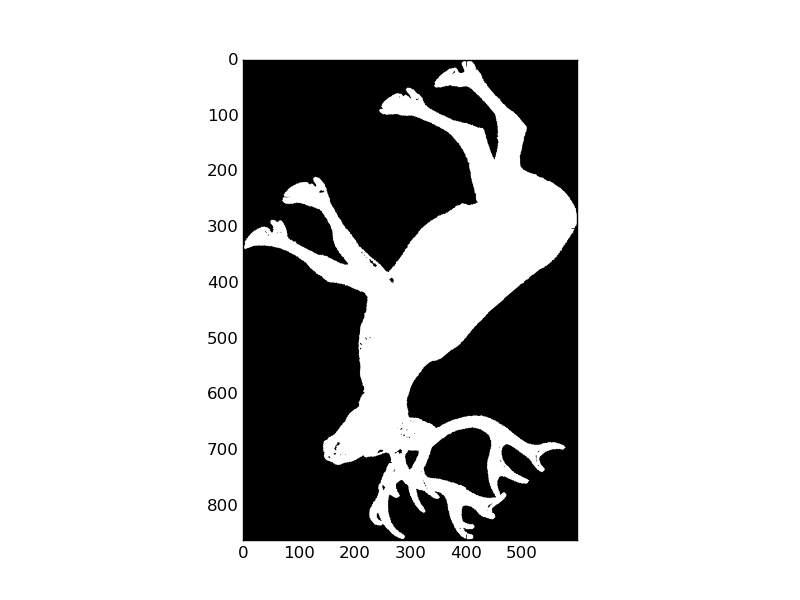
\includegraphics[scale=0.15]{rotate/220.png} \\
    0 degré & 30 degrés & 120 degrés & 220 degrés
  \end{tabular}
\end{center}

\begin{table}[H]
  \begin{center}
    \begin{tabular}{c | c c c c c c c c}
                & $\lambda_1$ & $\lambda_2$ & $\lambda_3$ & $\lambda_4$ & $\lambda_5$ & $\lambda_6$ & $\lambda_7$ & $\lambda_8$ \\ \hline
      0 degré    & 118.57 & 177.16 & 252.35 & 285.53 & 361.22 & 404.89 & 420.69 & 489.36 \\
      30 degrés  & 120.28 & 182.75 & 257.54 & 297.97 & 370.39 & 413.53 & 426.99 & 472.08 \\
      120 degrés & 120.29 & 182.88 & 266.09 & 308.13 & 372.66 & 414.83 & 428.60 & 472.21 \\
      220 degrés & 120.42 & 182.95 & 250.94 & 299.81 & 366.01 & 406.55 & 424.32 & 478.39 
    \end{tabular}
  \end{center}
  \caption{Valeurs propres associées à \texttt{deer-20.pgm} en fonctions de l'angle de rotation}
  \label{rot}
\end{table}

~\\
\underline{Bruit} Le bruit peut déformer le domaine de l'image et modifier par conséquent les valeurs propres. Cependant, les premières valeurs propres ($\lambda_1, \lambda_2, \lambda_3, \dots$) correspondent à la fondamentale et aux premières harmoniques, et donc aux composantes de la solution au Laplacien de Dirichlet de longueur d'onde élevé. Par conséquent, on peut s'attendre à ce qu'une déformation relativement faible du contour impacte peu ces valeurs (contrairement aux valeurs associées à des longueurs d'onde faibles). {\large \textcolor{red}{Vrai ?}} Par ailleurs, le redimensionnement systématique de l'image que l'on applique permet de gommer partiellement le bruit.

Afin de tester la robustesse au bruit, nous avons implémenté un modèle de bruit de Kanungo (pour un facteur de bruit $0 \leq a \leq 1$, tout point $x$ du domaine à distance $d$ du bord est colorié en noir avec probabilité $a^d$). La table \ref{bruit} démontre le faible impact du bruit sur les valeurs propres.

\begin{center}
  \begin{tabular}{c c c c}
    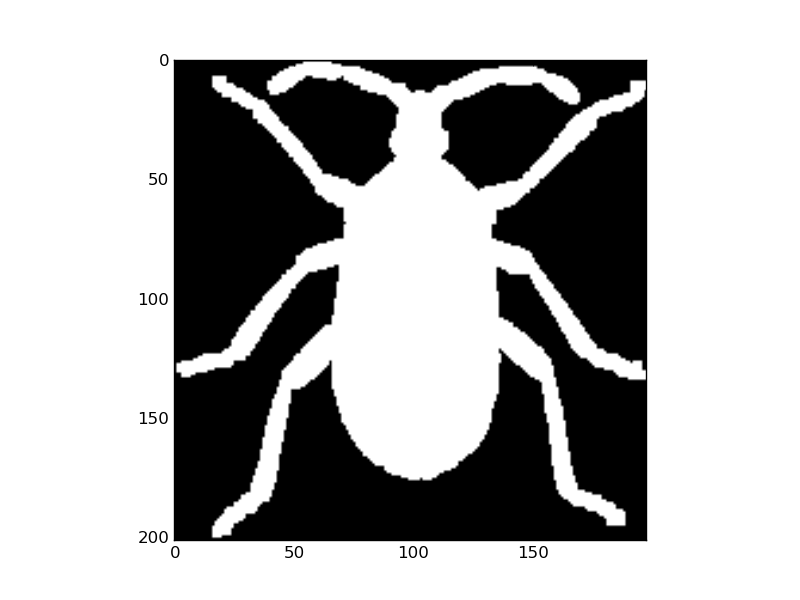
\includegraphics[scale=0.15]{noise/0.png} & 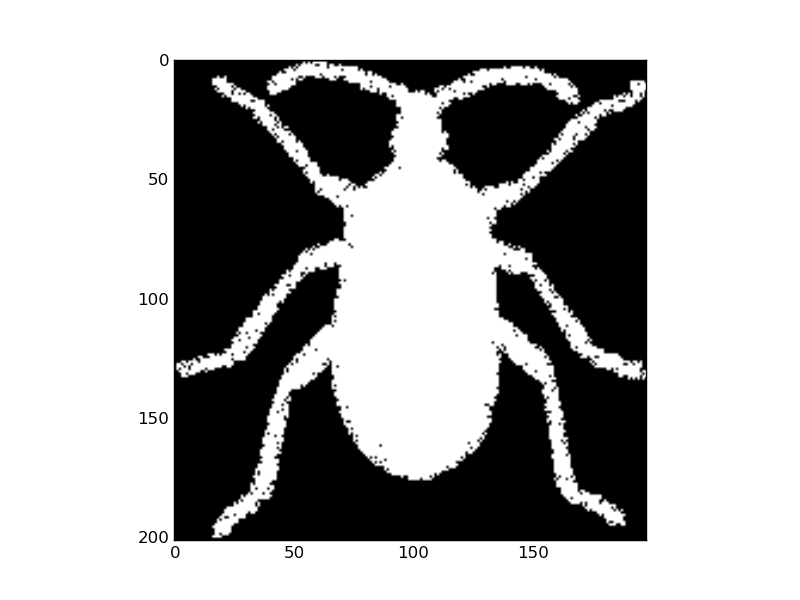
\includegraphics[scale=0.15]{noise/0_3.png} & 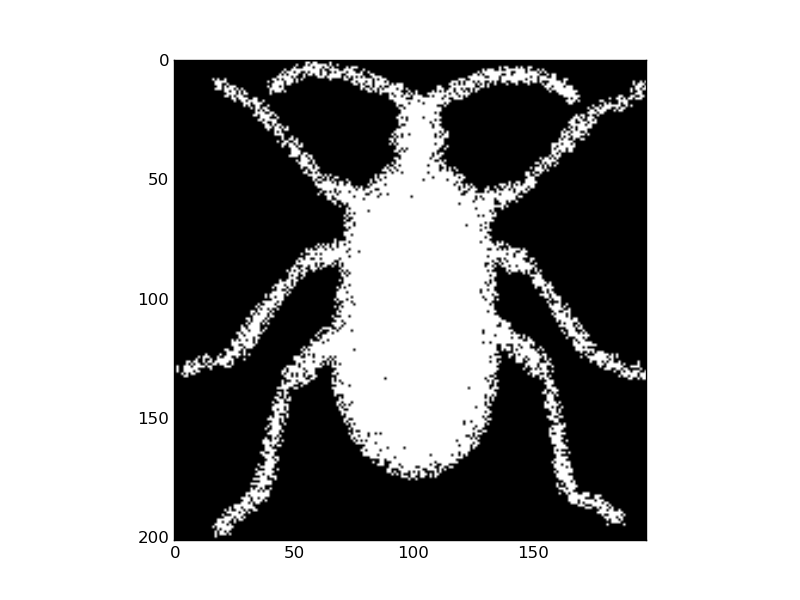
\includegraphics[scale=0.15]{noise/0_6.png} & 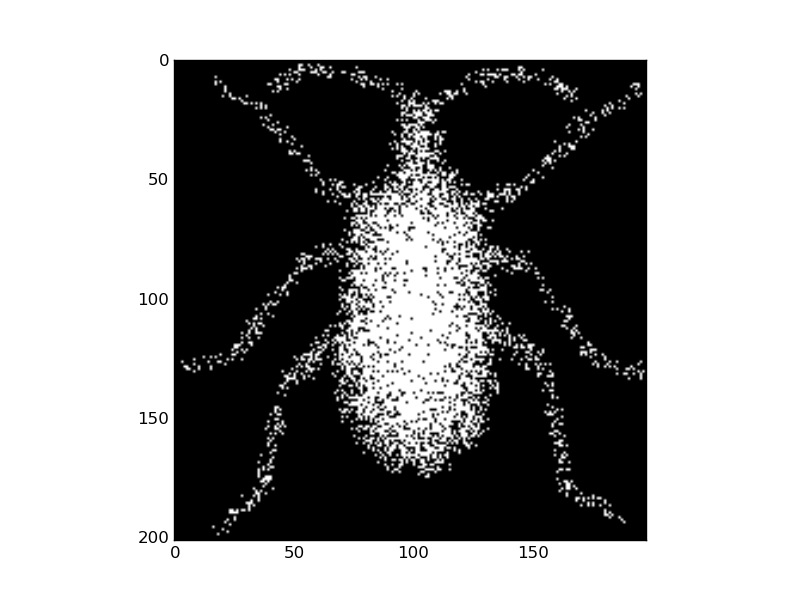
\includegraphics[scale=0.15]{noise/0_9.png} \\
    Bruit 0 & Bruit 0.3 & Bruit 0.6 & Bruit 0.9
  \end{tabular}
\end{center}

\begin{table}[H]
  \begin{center}
    \begin{tabular}{c | c c c c c c c c}
                 & $\lambda_1$ & $\lambda_2$ & $\lambda_3$ & $\lambda_4$ & $\lambda_5$ & $\lambda_6$ & $\lambda_7$ & $\lambda_8$ \\ \hline
      Bruit 0    & 83.93 & 153.41 & 258.76 & 263.10 & 353.64 & 378.19 & 495.73 & 500.11 \\
      Bruit 0.3  & 84.20 & 154.12 & 259.27 & 264.12 & 354.84 & 379.19 & 498.19 & 504.15 \\
      Bruit 0.6  & 84.42 & 155.22 & 262.05 & 264.96 & 355.90 & 388.19 & 503.35 & 514.37 \\
      Bruit 0.9  & 87.02 & 157.19 & 264.77 & 276.22 & 363.54 & 388.21 & 506.28 & 522.61  
    \end{tabular}
  \end{center}
  \caption{Valeurs propres associées à \texttt{beetle-13.pgm} en fonctions du facteur de bruit}
  \label{bruit}
\end{table}
%#############################################################################################################%
%#############################################################################################################%
%#############################################################################################################%

\section{Discussion}

%#############################################################################################################%
%#############################################################################################################%
%#############################################################################################################%

\section{Conclusion}

%#############################################################################################################%
%#############################################################################################################%
%#############################################################################################################%

\section*{Bonus}

Nous avons essayé de reconstruire un son à partir des valeurs propres du Laplacien de Dirichlet. Pour cela, à partir du spectre des valeurs propres $\{\lambda_1, \lambda_2, ...\}$ de l'image, on en déduit les fréquences pouvant se propager dans la cavité définie par l'image, de la forme $\{\alpha \sqrt{\lambda_1}, \alpha \sqrt{\lambda_2}, ...\}$, $\alpha$ étant une constante choisie de façon à ce que le spectre obtenu soit compris entre 100Hz et 2kHz.

En pratique, $\alpha = 40$, on ne retient que 3 valeurs propres. Enfin on associe la même puissance à chacune des 3 fréquences calculées.

On peut s'amuser à changer ces différents paramètres pour entendre des sons différents.



Afin d'entendre le son associé à l'image \texttt{beetle-11.pgm} par exemple, entrer : 
\begin{center}
  \texttt{python3 sound.py database/beetle-11.pgm}
\end{center}

Nous avons également développé un petit jeu, accessible par :
\begin{center}
  \texttt{python3 sound\_game.py}
\end{center}


Il s'agit de retrouver parmi les sons de plusieurs objets celui appartenant à la même catégorie qu'un motif de départ. 

%#############################################################################################################%
%#############################################################################################################%
%#############################################################################################################%

\bibliographystyle{alpha}
\bibliography{Biblio}
\nocite{*}

\end{document}